\documentclass[tesis.tex]{subfiles}

%\newcommand{\ol}{\overline{}}
%\newcommand{\ic}{independiente de contexto }
%\newcommand{\APND}{automáta de pila no determinístico }
%\newcommand{\APD}{automáta de pila determinístico }
%\newcommand{\fg}{grupo finitamente generado }
%\newcommand{\fp}{grupo finitamente presentado }
%\newcommand{\vl}{virtualmente libre}
%\newcommand{\WP}{\text{WP}(G, \Sigma)}
%\newcommand{\deriva}{\overset{*}{\Rightarrow_{\cal G}}}
%\newcommand{\cG}{ {\cal G} }



\begin{document}
	
\chapter{Grupos virtualmente libres.}
En este capítulo veremos como entran en juego las diferentes áreas de la matemática para definir de manera equivalente a los grupos virtualmente libres.

\begin{deff}
Un grupo $G$ finitamente generado es \blue{virtualmente libre} si existe un subgrupo libre $F$ tal que su índice en $G$ es finito.
\end{deff}

Veamos algunas propiedades elementales que cumplen todos los grupos \vl. 
Antes probemos algunos lemas sobre grupos.
\begin{deff}
	Sea $G$ un grupo y $H$ un subgrupo entonces el normalizador de $H$ en $G$ es el siguiente subgrupo
	\begin{equation*}
		N_G(H) = \{ g\in G : gHg^{-1} = H  \}
	\end{equation*}
\end{deff}

Denotaremos por $S= \{ g \in G :  gHg^{-1} \}$ al conjunto de conjugados del subgrupo $H$. 

\begin{lema}\label{lema_normalizador_conjugados}
	Si $G$ es un grupo \fg y $H$ es un subgrupo de índice finito entonces $N_G(H)$ tiene índice finito y más aún $[G:N_G(H)] = |S|$.
\end{lema}
\begin{proof}
	Para ver que tiene índice finito notemos que $H \le N_G(H)$ por lo tanto tenemos que 
	\[
		[G:N_G(H)] \le [G:H] < \infty.
	\]
	
	Para probar la otra afirmación definimos la siguiente función hacia los cosets a derecha del normalizador desde el conjunto $S$,
	\begin{align*}
		S  &\to  G/N_G(H) \\
		sHs^{-1} &\mapsto N_G(H)s
	\end{align*}
	Veamos que es biyectiva.
	
	Si $N_G(H)s = N_G(H)t$ entonces tenemos que esto sucede si y solo sí $st^{-1} \in N_G(H)$.
	Esto nos dice que por la definición del normalizador,
	\[
		st^{-1} H ts^{-1} = H \iff s^{-1}Hs = t^{-1}Ht
 	\]
 	y de esta manera obtenemos que la función está bien definida y es biyectiva.
\end{proof}

\begin{lema}\label{lema_indice_interseccion}
	Sea $G$ un grupo \fg \  y sean $K,H$ subgrupos de índice finito entonces $K \cap H$ es un subgrupo de índice finito.
\end{lema}
\begin{proof}
	Primero notemos que por el segundo teorema de isomorfismo para grupos tenemos que existe una biyección entre los siguientes conjuntos,
	\[
		KH / K \simeq K / K \cap H
	\]
	y en particular como $|KH / K| \le |G / K| < \infty$ por hipótesis obtenemos así que $|K / K \cap H| < \infty$.
	
	Finalmente por una propiedad de índices de subgrupos obtenemos lo siguiente
	\[
		[G:K\cap H] = [G:K][K: K \cap H]
	\]
	 y como ambos índices de la derecha son finitos por lo visto obtenemos que $K \cap H$ es un subgrupo de índice finito también tal como queríamos ver.
\end{proof}

\begin{lema}\label{lema_subg_fg}
	Sea $G$ un \fg y sea $H$ subgrupo de índice finito entonces $H$ es un \fg.
\end{lema}
\begin{proof}
	Sea $A = \{g_1, \dots, g_n\}$ conjunto finito de generadores de $G$.
	Sea $T =\{t_1, \dots, t_m\}$ conjunto transversal a derecha de $H$, esto es que $Ht_1, \dots, Ht_k$ son todos los cosets a derecha de $H$ sobre $G$.
	Supongamos que $t_1=1$ dado que es el representante del coset $H$.

	Dado $g_j$ generador de $G$ debe existir $h_{ij} \in H$ tal que $h_{ij}t_{k} = t_ig_j$ para cierto $t_k$.
	También debe existir $h_i \in H$ de manera que $ h_i t_{k} = g_i$ para cierto $t_k$.
	Veamos que el conjunto finito 
	\[
		B = \{ h_{ ij}  \}_{1 \le i,j \le n } \cup \{ h_i \}_{1 \le i \le n}
	\]
	 genera a $H$.
	
	Dado $h \in H$ tenemos que 
	\[
		h = g_{i_1}\dots g_{i_r}
	\]
	donde usamos el conjunto finito de generadores de $G$.
	
	Por lo visto anteriormente podemos escribir  $g_{i_1} = h_{i_1}t_{k_1}$ y entonces nos queda la siguiente escritura de $h$,
	\[
		h = h_{i_1}t_{k_1} g_{i_2}\dots g_{i_r}
	\]
	entonces usando que $h_{k_{1}i_{2}}t_{k_2} = t_{k_1}g_{i_2} $ llegamos a la siguiente escritura de $h$,
	\[
	h = h_{i_1}h_{k_{1}i_{2}}t_{k_2}\dots g_{i_r}.
	\]
	Repitiendo inductivamente este procedimiento llegamos a que $h =h_{i_1}h_{k_{1}i_{2}} \dots t_{k_r}$.
	Este $t_{k_r}$ tiene que ser $1$ porque justamente $h \in H$, por lo tanto tenemos $B$ es un conjunto finito de generadores de $H$.
\end{proof}


Con esto podemos probar estos resultados elementales de grupos \vl.

\begin{prop}\label{prop_vls}
	Para todo grupo $G$ \vl \ valen las siguientes propiedades.
	\begin{enumerate}
		\item Si $F$ es un subgrupo libre de índice finito entonces podemos tomarnos otro subgrupo $F'$ de manera que sea normal, libre y de índice finito.
		\item Si $H$ es un subgrupo de $G$ de índice finito entonces $H$ también resulta ser \vl.
	\end{enumerate}
\end{prop}

\begin{proof}
	\begin{enumerate}
		\item Si $G$ es virtualmente libre y $F$ es un subgrupo libre tenemos que la cantidad de conjugados de $F$ es finita por el lema \ref{lema_normalizador_conjugados}.
		Por lo tanto podemos considerar el siguiente subgrupo normal
		\[
		F' = \bigcap_{g \in G} gFg^{-1}
		\]
		donde la cantidad de grupos que estamos intersecando es finita y es normal por construcción.
		Veamos que $F'$ nos sirve. 
		Para ver que tiene índice finito nos alcanza con usar el lema \ref{lema_indice_interseccion} e inducción para que valga para una intersección finita arbitraria.
		Como tiene índice finito usando \ref{lema_subg_fg} sabemos entonces que es un \fg.
		Finalmente notemos que es libre por el resultado \ref{coro_niels_sch} que nos dice que todo subgrupo de un grupo libre es libre, en particular al ser $F'$ subgrupo de $F$ que es libre obtenemos que $F'$ es libre tal como queríamos ver.
		
		\item Por el lema \ref{lema_subg_fg} obtenemos directamente que $H$ es \fg.
		Si $F$ es un libre de índice finito en $G$ podemos tomar $H \cap F$ que es libre por ser subgrupo de un libre de acuerdo al resultado \ref{coro_niels_sch}.
		El índice resulta ser finito puesto que 
		\[
			[H:F\cap H] \le [G:F] < \infty.
		\]
	\end{enumerate}
\end{proof}

\begin{obs}\label{obs_presentacion_vl}
	Dado $G$ \vl \ vamos a construirnos una presentación en particular.
	
	Como es un grupo \vl \ tenemos $F$ subgrupo libre que podemos tomarlo normal y $G/F$ grupo finito de manera que podemos escribir a $G$ como una extensión de estos dos grupos por medio de la siguiente forma
	\begin{center}
		\begin{tikzcd}
			1 \arrow[r] & F \arrow[r, "\iota"] & G \arrow[r, "\pi"] & G/F \arrow[r] & 1
		\end{tikzcd}
	\end{center}
	
	Consideremos que $F$ es libre generado por $Y = \{ y_1, \dots, y_n \}$.
	Por otro lado sea $G/F = \{ b_i : 1 \le i \le m \}$ todos los elementos de este conjunto finito.
	Elegimos un transversal a derecha $T = \{ t_1, \dots, t_m \}$ de manera que $\pi(t_i)= b_i$ y $t_1 = 1$.
	
	Dado que es un transversal tenemos que se deben cumplir las siguientes dos relaciones para $y_j \in Y$ y $t_i,t_j,t_k \in T$. 
	\begin{enumerate}
		\item $t_iy_jt_i^{-1} = u_{ij}$ donde $u_{ij} \in F$ usando que $F$ es normal.
		\item Si tenemos que $b_ib_j = b_k$ entonces $t_it_j = z_{ij}t_k$ donde $z_{ij} \in F$ usando que $(Ht_i)(Ht_j) = Ht_k$.
	\end{enumerate}
	
	Afirmamos que la siguiente es una presentación finita de $G$.
	\[
		\langle W \mid R \rangle =  \langle y_1, \dots, y_n, t_1, \dots, t_m \mid t_iy_jt_i^{-1} = u_{ij},  t_it_j = z_{ij}t_k \rangle.
	\]
	Sea el grupo que genera este presentación $H$ y sea $F'$ el grupo libre sobre sus generadores.
	
	Notemos que $W =Y \cup T$ genera a $G$ porque justamente $F$ es libre y generado por $Y$ y $T$ es un conjunto transversal finito porque $F$ tiene índice finito en $G$.
	Esto nos dice que tenemos un epimorfismo de grupos de $F'$ en el grupo $G$.
	
	Toda relación de $G'$ la cumple el grupo $G$ por la elección que tomamos, de esta manera tenemos un epimorfismo de grupos $\ol \varphi$ tal que hace conmutar al siguiente diagrama,
	
	\begin{center}
		\begin{tikzcd}
			F' \arrow[dd] \arrow[rr, "\varphi"]          &  & G \\
			&  &   \\
			H \arrow[rruu, "\overline \varphi"', dashed] &  &  
		\end{tikzcd}
	\end{center}
	
	El grupo  $G$ es tal que a toda palabra $w$ en sus generadores la podemos llevar a que sea de la pinta
	\[
		w = yt
	\]
	donde $y \in F$ reducida y $t \in T$ es alguno de los transversales. 
	Para llegar a esto hacemos el mismo procedimiento que hicimos en la demostración del lema \ref{lema_subg_fg}.
	
	De esta manera una palabra es trivial si y solamente si $y=1$ y $t=1$. 
	Esto nos dice que $\varphi(w) = 1$ si y solamente si $w=1$. 
	Concluimos así que $\ol \varphi$ es un isomorfismo de grupos tal como queríamos ver y por lo tanto  $\langle W \mid R \rangle$ resultó ser una presentación de $G$.
	
\end{obs}
\medskip

Veamos ahora unos ejemplos y contrajemplos de grupos \vl s.

\begin{ej}
Veamos algunos ejemplos elementales de grupos que son de esta familia y algunos que no lo sean.
\todo[inline]{Agregar la construcción de la presentación de los grupos \vl.}
\begin{enumerate}	
	\item Cualquier extensión de un grupo libre por un grupo finito es un grupo virtualmente libre,
	\[
		1 \to F \to G \to K \to 1
	\]
	donde $K$ es un grupo finito y $F$ es un grupo \fg libre.
	En particular esto nos da los casos más elementales de productos directos y semidirectos, esto es $G= F \times K$ o bien  $G = F \ltimes K$.
	En este capítulo veremos que todo grupo \vl \ podemos considerarlo como un subgrupo de una extensión de este tipo.
	
	\item El ejemplo más sencillo de un grupo que no es \vl \ es $\ZZ \times \ZZ$.
	La primera observación es que al ser abeliano si tiene un subgrupo libre necesariamente tiene que ser isomorfo a $\ZZ$.
	
	Nos alcanza con ver que no es virtualmente $\ZZ$.
	Sea $F$ un subgrupo que es isomorfo a $\ZZ$.
	Sea $(n,m) \in \ZZ \times \ZZ$ el generador de $F$.
	Probaremos que $\ZZ \times \ZZ / F$ tiene orden infinito.
	Para eso consideraremos $(p,q) \in \ZZ \times \ZZ$	tal que $p,q$ son primos distintos y ambos coprimos con $m,n$.
	Veamos que $[(p,q)] \in \ZZ \times \ZZ / F$ tiene orden infinito.
	Si no lo fuera deberían existir $\alpha, \beta \in \ZZ$ de manera que 
	\begin{align*}
		\alpha (p,q) = \beta(n,m) 
	\end{align*}
	
	como todos son coprimos entre sí esto nos dice que $p \mid \beta$ y similarmente que $q \mid \beta$, por lo que tenemos que $q \mid \alpha$ y $p \mid \alpha$.
	Esto nos dice que se pueden escribir de esta manera
	\begin{align*}
		\alpha = p^{r_1} q^{s_1} \gamma_1 \\
		\beta = p^{r_2} q^{s_2} \gamma_2
	\end{align*}
	con $r_i, s_i > 1$ para $i=1,2$.

	Finalmente como 
	\[ 
		\alpha p = \beta n
	\]
	tenemos que $r_1+ 1 = r_2$ pero por otro lado como
	\[
		\alpha q  = \beta m
	\]
	acá tenemos que al ser $m$ coprimo con $p$ luego la multiplicidad de $p$ en la descomposición en primos de lo que está a la izquierda es $r_2 - 1 \le 0$ mientras que lo que está a la derecha es $r_2$.
	Esto es una contradicción que vino de suponer que $[(p,q)] \in \ZZ \times \ZZ / F$ tenía orden finito por lo tanto tenemos que $\ZZ \times \ZZ$ no puede ser \vl.
	
\end{enumerate}
\end{ej}






\section{Grupos independientes de contexto.}
 
 En esta sección definiremos una familia de grupos que veremos más en adelante que coincide con los grupos \vl.
 Como corolario de la proposición \ref{prop-cono-wp} y de saber que los lenguajes \ic \ forman un cono \ref{ic-cono} la siguiente definición no depende del conjunto de generadores.
 \medskip
\begin{deff}
	Si $G$ es un grupo \fg tal que para ciertos generadores $\Sigma$ resulta que $WP(G, \Sigma)$ es independiente de contexto entonces diremos que $G$ es un \blue{grupo \ic }.
\end{deff}


\begin{ej} Consideremos los siguientes ejemplos.	
	\begin{enumerate}[E1.]
		\item 
		Dado $F$ grupo libre de rango finito supongamos generado por el conjunto finito $X$. 
		Sea  $Y = X \cup X^{-1}$ el conjunto de generadores simétrico de $X$. 
		Probemos que $\text{WP}(F,Y)$ es un lenguaje independiente de contexto.
		
		Consideremos el siguiente autómata de pila,
		\[
			M = (\{ 1 \}, Y, Y, \delta, 1, \{1\}).
		\]
		
		Por como lo definimos tiene un solo estado y el alfabeto tanto de entrada como el de la pila que usa es el conjunto de generadores $Y$.
		La función de transición $\delta$ está definida de la siguiente manera,
		\[
		\delta(1, y_i, u)=\left\{
		\begin{array}{ll}
			(1 , u )  &\ \text{si} \ a = 1  \\
			(1, y_i \cdot u') &\ \text{si} \  u = y_jw'  \\
		\end{array}
		\right.
		\]
		donde al apilar hacemos la multiplicación $y_i \cdot u$ en el grupo libre $F$.
		
		Consideremos el lenguaje aceptado por pila vacía, esto es
		
		\[
		{\cal L }(M) = \{  y \in Y^* \mid (y,1,1)   \vdash^*  (1, 1, 1)  \}.
		\]
		
		Notemos que ${\cal L }(M) = \text{WP}(F,Y)$ porque justamente en la pila apilamos lo que vamos leyendo de izquierda a derecha y desapilamos cuando leemos el inverso del generador que está en el tope de la pila.
		Esto es que desapilamos cuando un generador aparece después de su inverso en la palabra.
	
		
%		Dado un grupo libre $F$ veamos cómo construir un automáta $\cal M$ tal que acepta su problema de la palabra. 
%		
%		Pensemos un \APND que tenga dos estados. Uno inicial que también va a ser final para poder aceptar la palabra vacía que corresponde al elemento 1 de nuestro grupo y otro estado para las palabras que no están en el problema de la palabra.
%		Para eso la idea es tener en la pila lo que fuimos leyendo de nuestra palabra hasta el momento visto como un elemento en el grupo. 
%		Esto es, cada vez que leemos una letra de la palabra ver de multiplicarla como un elemento en el grupo con lo que tenemos en el tope de la pila. 
%		Eventualmente cuando hayamos recorrido la palabra entera debería quedarnos una palabra en la pila que queremos que sea exactamente $1$ y esto es lo mismo que pedir que sea aceptada por pila vacía. 
%		Entonces este automáta lo podemos representar de la siguiente manera:	
%		
%		\begin{center}
%			\begin{tikzpicture}[->,>=stealth',shorten >=1pt,auto,node distance=4.5cm,
%				scale = 1.15,transform shape]
%				
%				\node[state,accepting,initial] (1') {$1'$};
%				\node[state] (1) [right of=1'] {$1$};
%				
%				\path (1') edge[bend left]              node {} (1)
%				(1) edge[bend left]              node {} (1');
%			\end{tikzpicture}
%		\end{center}
%		
%		
%		Donde las transiciones del estado 1' a 1 son todas las transiciones en las cuales la letra que estamos por leer no es la inversa de lo que esté al tope de la pila. Por otro lado las transiciones del estado 1 al estado 1' son todas las que lo que leemos es justamente el inverso de lo que está al tope de la pila.
		
		\item 	$\ZZ \times \ZZ$ no es un grupo independiente de contexto.
		Si tomamos los siguientes generadores como monoide $\Sigma = \{ a,b,c \}$ tal que tenemos un morfismo de monoides $\pi: \Sigma^* \to \ZZ \times \ZZ$ dado por $\pi(a)=(1,0), \pi(b)=(0,1), \pi(c)=(-1,-1)$.
		Bajo esta presentación 
		\[
		WP(\ZZ \times \ZZ, \Sigma) = \{ w \in \Sigma^*  : \ \exists n \in \NN, \ |w|_a = |w|_b = |w|_c = n \}.
		\]
		Este lenguaje no es independiente de contexto.
		Para eso usemos el lema del pumping \ref{pumping} para probarlo por contradicción.
		Si fuera \ic debería existir una constante $n \ge 0$ tal que hace valer las hipotesis del lema.
		Consideremos la palabra $w = a^n b^n c^n \in WP(G, \Sigma)$.
		Si tenemos una factorización 
		\[
		uvwxy = a^nb^nc^n
		\]
		 si $|vwx| \le n$ implica que no todas las letras aparecen en $vwx$.
		Supongamos que la letra que no aparece es $c$.
		Por otro lado como $|vx| \le 0$ esto nos dice que al menos una letra aparece en la subpalabra $vx$.
		Si tomamos $i=0$ notemos que la palabra $uwy \in WP(G,\Sigma)$ pero esto es una contradicción porque la cantidad de $c$ en esta palabra es mayor que de $a$ o $b$.
		
	\end{enumerate}
	
\end{ej}

\begin{obs}\label{palabras-wp}
	Si tenemos un grupo $G$ tal que es independiente de contexto consideremos $\cal G$ gramática que genera al lenguaje del problema de la palabra, $\WP = L(\cal G)$.
	Si $A$ es una de las variables de esta gramática podemos obtener el lenguaje $L_A$ de palabras generadas a partir de esta variable, donde
	\[
	L_A = \{ w \in \Sigma^*  \ | \ A \deriva w  \}.
	\]
	Veamos que si $v,v' \in L_A$ entonces $v =_G v'$, es decir son el mismo elemento vistos en el grupo $G$. 
	Para eso si tenemos una derivación que en algún momento llega a $S \deriva \beta A \gamma \deriva uvw$ también tenemos otra derivación que deriva en $S \deriva \beta A \gamma  \deriva uv'w$. 
	Es decir que $uvw, u'v'w' \in \WP$ por lo tanto 
	\begin{equation*}
		uvw =_G 1 =_G uv'w \implies v =_G v'
	\end{equation*}
	tal como queríamos ver.
\end{obs}



Una pregunta natural es intentar entender la relación entre la clasificación del lenguaje del problema de la palabra de un grupo dado y las distintas familias de grupos que le corresponden. 
La siguiente demostración generaliza la construcción del ejemplo del problema de la palabra de un grupo libre.


\begin{teo}\cite{muller1985theory}
	Todo grupo virtualmente libre es independiente de contexto.
\end{teo}

 
\begin{proof}
	Sea $G$ grupo \vl  \ y consideremos una presentación $\langle W  \mid  R \rangle$ como la que construimos en la observación \ref{obs_presentacion_vl}.
	Veamos de construir un autómata de pila de manera que acepte al lenguaje $\text{WP}(G,W)$.
	
	Vamos a definir un autómata de pila con estados de control finitos que sabemos que es equivalente a un autómata de pila no determinístico por la observación \ref{}.
	
	
	Nuestro autómata lo definimos así: 
	\[
	{\cal M }= (T, W , Y, \delta, 1, \{1\}, K)
	\]
	donde $T$ es el conjunto de los transversales que tomamos para la presentación de $G$ y van a ser los estados del autómata.
	El alfabeto de entrada es $W$ el conjunto de generadores del grupo.
	El alfabeto de la pila es $Y$ que es el conjunto de generadores del subgrupo libre $F$.
	Nuestro estado inicial que también es final corresponde a $1$ que es uno de los elementos del transversal.
	La constante que tomamos es $K = \max |u_{ij},\ z_{ijk}|$ donde $1 \le i,j,k  \le n$. 
	
		
	Ahora podemos definir la función de transición.
	Si tenemos que $ t_j y_i = u_{ij} t_j $ y que $ t_it_j = z_{ijk}t_k $ luego consideremos la siguiente definición,
	\begin{align*}
		\delta(y_iw',t_j, v) &= (w', t_j, u_{ij} \cdot v) \\
		\delta(t_iw',t_j, v) &= (w', t_k, z_{ijk} \cdot v) \\
		\delta(1, t_j, v) &= (1, t_j, v) \\
	\end{align*}
	donde en la pila al apilar hacemos el producto en el grupo libre para ir reduciendo la palabra de la pila.
	Sabemos que hacemos tantas reducciones como $|u_{ij}|$ o bien $| z_{ijk}|$ y ambos valores están acotados por la constante $K$.
	Esto nos dice que está bien definido.
	
	
	Consideremos el lenguaje aceptado por pila vacía y estado final a la vez,
	
	\[
		{\cal L }(M) = \{  w \in W^* \mid (w,1,1)   \vdash^*  (1, 1, 1)  \}
	\]
	Debemos ver que el autómata acepta justamente al lenguaje que queremos. 
	Esto es que $ {\cal L }(M) = \text{WP}(G,W) $ 
	
	
	Dada una palabra $w \in W^*$ por como es esta presentación sabemos que se puede escribir como $w = vt$ donde $v \in F$ reducida y $t \in  T$. 
	De esta manera $w \in \text{WP}(G,W)$ si y solo si $v=1, t=1$.
	Notemos que el autómata en toda transición no hace más que reescribir la cadena de izquierda a derecha tal como hicimos en la observación \ref{obs_presentacion_vl}.
	Esto es que cuando termina de consumir la cadena de entrada llegamos a la configuración $(1, t_i, v)$ es decir que $w = vt_i$.
	Por lo tanto como aceptamos por estado final y pila vacía esto nos dice que $w \in \text{WP}(G,W)$ si y solo sí $w \in {\cal L}(M)$.
		
	Con esto probamos que los grupos virtualmente libres son \ic usando la equivalencia \ref{teo_ic_apnd}.
	
	
%	Fijemos entonces un subgrupo libre de índice finito $F$ que lo podemos tomar de manera que sea normal por la proposición \ref{prop_vls}. 
%	Sea $T$ conjunto transversal a derecha de $G/F$ que sabemos que es finito. 
%	Consideremos al conjunto  $\Delta = \Sigma \cup \Sigma^{-1} \cup T$ de generadores de nuestro grupo porque en particular sabemos que $\Sigma$ generaba .
	
%	Recordemos por \ref{} que para todo grupo virtualmente libre tenemos un sistema de reescritura convergente dado por 
%	\[
%	S = \{ ab \to w(a,b)r  \}
%	\] 
%	donde $w(a,b) \in F_\Sigma$ es una palabra reducida y $r \in R$ tal que $ab = w(a,b)r$. Vamos a usar este sistema para construirnos la función de transición de nuestro automáta. 
%	
%	Nuestro automáta lo definimos así 
%	\[
%	{\cal M }= (Q,\Delta, Z, \delta, q_0, F)
%	\]
%	donde los estados $Q$ se corresponden a $R \cup R'$ siendo $R'$ una copia de $R$. 
%	Para el alfabeto de la pila consideramos solamente el alfabeto del subgrupo libre y otra vez agregamos otras copias de manera que nuestro alfabeto para la pila es $Z = \Sigma \cup \Sigma^{-1} \cup (\Sigma \cup \Sigma^{-1})^{'}$. 
%	Nuestro estado inicial es $q_0 = 1' \in R'$ es decir el $1$ de la copia. Nuestro conjunto de estados finales contiene solamente al estado inicial $F=q_0$. 
%	Notemos a su vez a $m = \max {|w(r,a)|}$ para $r \in R, a \in \Delta$ que es finito porque es el máximo de longitudes de finitas palabras. 
%	Cuando tengamos una ecuación en término de las copias la vamos a considerar como el elemento que representa en el grupo. 
%	La utilidad radica en poder tener un automáta más declarativo en cuanto a los nombres de los estados. 
%	Nuestra función de transición entonces funciona de la siguiente manera si no tenemos nada en la pila
%	
%	\begin{align*}
%		(r'a,w(r'a)s) \in \delta  \ \ \ \text{para} \ \  s \in R \ \ \text{tal que} \ r'a=w(r',a)s \ \ \text{y} \ \ w(r',a) \neq 1  \\
%		(r'a,s') \in \delta  \ \ \text{para} \ \  s \in R \ \ \text{tal que} \ r'a=s.  \\ 
%	\end{align*}
%	
%Si la palabra reducida $w(r',a)$ es distinta de la identidad entonces pasamos a los estados que le corresponden a $R$ mientras que en el otro caso nos quedamos en los estados de la copia $R'$. 
%En particular como el estado inicial es $1' \in R'$ luego siempre que tengamos la pila no vacía vamos a estar en algún estado $r \in R$. 
%Repliquemos esta idea también para el caso que que tengamos algo en la pila,
%	
%	\begin{align*}
%	(xra,ys) \in \delta \ \ \text{para} \ \  s \in R, x,y \in (\Sigma \cup \Sigma^{-1})^m & \ \  \text{tal que} \ ra=w(r,a)s  \\ & \ \ \text{e} \ \ y \ \text{es la forma reducida de} \ \ xw(r,a)  \\
%	(xra,s') \in \delta\ \ \text{para} \ \  s' \in R', x,y \in (\Sigma \cup \Sigma^{-1})^m & \ \  \text{tal que} \ ra=w(r,a)s'  \\ & \ \ \text{e}  \ \ xw(r,a)  \ \text{se reduce a 1}. \ \  \\ 
%	\end{align*}
%	En este caso la función de transición cuando tenemos algo en la pila lo que va haciendo es lo mismo que antes y solo pasa a los estados que corresponden a $R'$ cuando la palabra que nos queda la pila vacía. 
%	
%	De esta manera notemos que en particular es un automáta especial determinístico considerando que la transición es determinística porque el sistema de reescritura es convergente por lo que hay una única palabra reducida. 
%	Por otro lado como el único estado que acepta es el estado inicial y la única manera de llegar a cualquier estado en $R'$ es con la pila vacía luego el automáta acepta por pila vacía y estado final a la vez.
\end{proof}

%\begin{obs}
%	Dado un grupo \vl \ con presentación $\langle W \mid R \rangle$ obtuvimos que el lenguaje $WP(G, W)$ no solo es aceptado por un autómata de pila no determinístico sino que es aceptado por uno determinístico especial tal como en la definición \ref{}.
%	Esto nos dice que sus propiedades algorítmicas son aun mejores. 
%	Siguiendo la referencia \cite{} tenemos que el problema de la palabra se puede resolver en $O (n^2)$ usando algoritmos estándares como...
%\end{obs}


\section{Grafos de Cayley.} \label{seccion_treewidth}

Un grafo en esta sección va a estar definido por su conjunto de vértices $V(X)$ y por uno de aristas $E(X) \subseteq V(X) \times V(X)$.
En particular las aristas no van a estar dirigidas y no tomaremos a $(v,v)$ como una arista para ningún $v \in V(X)$.

\begin{deff}
	Sea $G$ un \fg y $\Sigma$ un conjunto de generadores como grupo. 
	Supongamos que $1 \notin \Sigma$.
	Definimos el \blue{grafo de Cayley} $\Gamma = \text{Cay}(G,\Sigma)$ como el grafo que tiene como vértices $V(\Gamma) = G$ y aristas $(g,h) \in E(\Gamma)$ sii $h=ga$ para ciertos $g,h \in G$ y $a \in \Sigma \cup \Sigma^{-1}$. 
\end{deff}

Para una arista $(g,ga)$ llamaremos la \emph{etiqueta} al generador $a$.
Extendemos esta definición a caminos sobre el grafo para obtener una palabra en el monoide $\Sigma^*$.
Este grafo por como lo definimos no tiene aristas múltiples ni tampoco tiene bucles.
Dado que $\Sigma$ es un conjunto d tenemos que el grafo $\Gamma$ es conexo.

El grafo de Cayley lo podemos ver como un espacio métrico justamente si hacemos que todas las aristas sean isométricas a $[0,1]$. 
Esto es que $d(g,ga) = 1$ para todo $g \in G, a \in \Sigma \cup \Sigma^{-1}$. 
Un camino $\alpha = g_0 \dots g_n$ es una \emph{geodésica} si $d(g_i,g_j) = j-i$ para todo $i,j \in [0,n]$.


Un \emph{árbol} es un grafo conexo y sin ciclos. 
En particular los árboles vistos como espacios métricos resultan ser \emph{únicamente geodésicos}. 
Esto es que dados $v,w$ dos vértices existe una única geodésica $\gamma:[0,1] \to T$ tal que $\gamma(0)=v$ y $\gamma(1)=w$.

%\begin{ej}
%	Sea $\mathbb F_2 = \langle a, b \rangle$ el grupo libre en $a,b$. Su grafo de Cayley para estos generadores tiene la siguiente pinta,
%	\bigskip
%	\begin{center}
%	\begin{tikzpicture}
%	\draw l-system [l-system={cayley, axiom=[A] [+A] [-A] [++A], step=2.35cm, order=3}];
%	\end{tikzpicture}
%	\end{center}
%	
%	
%	 Notemos que este grafo resulta ser un árbol y esto es algo que vale en general para todos los grupos libres cuando miramos respecto a sus generadores canónicos.
%\end{ej}

Como todo grupo libre es tal que sus grafos de Cayley resultan ser árboles por un resultado clásico de Serre, ver \cite{}.
Es razonable pensar que todo grupo virtualmente libre es tal que su grafo de Cayley se parezca a un árbol. 
La primera noción que podemos tomar para modelizar esto es el de tener un treewidth finito.

\begin{deff}\label{desc-arbol}
	 Una \blue{descomposición en un árbol} de un grafo $X$ es un árbol $T$ y un mapa 
	 \[
	 X: V(T) \to {\cal P}(V(X))
	 \]
	  que denotaremos $X_t$ para cada vértice $t \in V(T)$. 
	  Le vamos a pedir que cumpla las siguientes condiciones:
	\begin{enumerate}
		\item[\textbf{T1.}] Para todo vértice $v \in V(X)$ debe existir $t \in V(T)$ tal que $x \in X_t$. 
		\item[\textbf{T2.}] Para toda arista $e$ entre dos vértices $v,w \in V(X)$ debe existir $t \in V(T)$ tal que $v,w \in X_t$.
		\item[\textbf{T3.}] Si $v \in V(X)$ es tal que $v \in X_t \cap X_s$ luego $v \in X_r$ para todo $r$ en la geodésica que va desde $s$ a $t$ dentro de $T$. En otras palabras esto es que $\{ t \in V(T) :  v \in X_t \}$ forma un subárbol. 
	\end{enumerate} 
\end{deff}
\smallskip

La idea de la descomposición es que los \emph{bolsones} $X_t \in {\cal P}(V(T))$ no tengan muchos vértices si es que queremos modelizar que el grafo se parezca a un árbol. Esto nos conduce a la siguiente definición.

\begin{deff}
El \blue{bagsize} de una descomposición en un árbol $T$ de un grafo $X$ es el siguiente valor:
	\begin{equation*}
		bs(X,T) = \{ \sup |X_t|, \ t \in V(T) : T \ \text{descomposición de} \ X  \} - 1
	\end{equation*}
Un grafo $X$ tiene \blue{treewidth finito} si existe una descomposición en un árbol de bagsize finito.	
\end{deff}
\begin{ej}\label{desc-arbol-arbol}
 En particular si el grafo $X$ es un árbol notemos que tiene treewidth exactamente igual a 1.
 Una manera de probarlo es tomar $T$ la subdivisión baricéntrica de $X$. 
 Este es el siguiente árbol que tiene como vértices a 
 \[
 V(T) = \{ s \ | \ s \in V(X)  \lor s \in E(X) \}.
 \]
 Tomamos todos los vértices de $X$ y los agregamos a los de $T$ y agregamos un vértice por cada arista del grafo $X$.
 Finalmente las aristas están formadas por 
 \[
 E(T) = \{  (s,t) \ | \ t \subset s \ \lor s \subset t \}
 \]
 agregamos una arista entre cada par de vértices de $T$ tales que uno se corresponde con un vértice de $X$ y el otro con una arista que lo contiene en $X$. 
%Por cada arista del grafo $e \in E(X)$ donde $e=xy$ con $x,y \in V(X)$ agregamos un vértice $v_e \in V(T)$ tal que definimos para que $xv_e, v_ey \in E(T)$.
 
 
 La descomposición que tomamos entonces es la siguiente. 
 Por cada $t \in V(T)$ tenemos ya armados los bolsones por la construcción que hicimos. 
 Esto es que:
 \begin{itemize}
 	\item Si $t$ es un vértice que ya estaba en $V(X)$ entonces $X_t = \{ t \}$. 
 	\item Si $t$ lo agregamos por una arista $(x,y) \in E(X)$ entonces $X_t = \{ x,y  \}$.
 \end{itemize}
Por como los definimos es evidente que $|X_t| \le 2$ para todo $t \in V(T)$.
De esta manera si vemos que se trata de una descomposición en un árbol tendremos probado que $bs(X,T) = 1$ tal como queríamos ver.

Finalmente veamos que se trata de una descomposición. Corroboremos que cumple las tres condiciones necesarias.
\begin{enumerate}
	\item[\textbf{T1.}] Todo vértice $v \in V(X)$ lo podemos ver como uno en $T$. Su bolsón asociado $X_v$ lo tiene como único elemento por la construcción de esta descomposición.
	\item[\textbf{T2.}] Si $xy \in E(X)$ entonces tenemos un vértice $t\in V(T)$ tal que $X_{t} = \{ x,y \}$. 
	\item[\textbf{T3.}] Sea $x \in X_t \cap X_s$. 
	Por como armamos los bolsones, uno de estos dos tiene que corresponderse con una arista de $X$.
	Supongamos que $X_t$ tiene esa pinta entonces $X_t = \{ x,y\}$ para cierto vértice $y \in V(X)$.
	
	En el caso que $X_s = \{ x \}$ la geodésica que podemos tomar entonces es $st$ puesto que $s$ se corresponde con el vértice $x$ y sabemos que existe una arista $st \in E(T)$ porque justamente $t$ se corresponde con una arista en $X$ que contiene a $x$.
	
	En el caso que $s \in V(T)$ sea tal que el bolsón $X_s$ se corresponda con los vértices que aparecen en una arista debería ser del tipo $X_s = \{x,z\}$ para cierto $z \in V(X)$. 
	Si miramos la geodésica sobre $T$ entre ambos vértices no es más que el siguiente camino $tvs$ donde $v \in V(T)$ es el vértice que está tanto en el árbol original $X$ como en la subdivisión baricéntrica $T$.
	Esto es que $X_v = \{ x \}$.
	De esta manera $x$ está en todos los bolsones correspondientes a la geodésica sobre $T$ tal como queríamos ver.	
\end{enumerate}
\end{ej}


% [Creo que está bastante mal esto. Si lo tengo que usar más en adelante repensarlo bien.]
%	\begin{obs}
%	Si un grafo $\Gamma$ tiene treewidth finito podemos tomarnos otra descomposición tal que siga siendo de treewidth finito pero los bolsones de la descomposición sean conexos. 
%	Si algún bolsón no es conexo agregamos todos los vértices del grafo que estén en la geodésica que une las componentes conexas. 
%	Haciendo esto la descomposición sigue siendo finita aunque el tamaño de los bolsones puede aumentar considerablemente.
%	\end{obs}

\begin{prop}\label{prop-camino-desc}
	Sea $\Gamma$ grafo tal que tiene una descomposición en un árbol $T$.
	Sean $X,Y,Z$ bolsones tales que el vértice correspondiente a $Z$ en el árbol $T$ está en la geodésica que va de $X$ a $Y$. 
	Sean $x \in X, y \in Y$ tales que $x = x_0 \dots x_n=y$ es algún camino en $\Gamma$ conectándolos.
	Entonces debe existir algún $ 0 \le i \le n$ tal que $x_i \in Z$. 
\end{prop}

\begin{proof}
	Vamos a demostrarlo haciendo inducción en la longitud $n$ del camino. 
	El caso base es que $n = 0$ por lo tanto $x=y$. 
	En este caso por ser una descomposición en un árbol tenemos que usando la tercer propiedad que $x \in Z$ también.
	
	Para el paso inductivo tomemos $X'$ bolsón que contiene tanto a $x$ como a $x_1$ que sabemos existe por ser una de las propiedades de las descomposiciones en árboles.
	Si este bolsón $X'$ es $Z$ ya está porque nos alcanza con tomar $i=1$ de manera que $x_1 \in Z$.
	En el caso que esto no ocurra miramos el camino de longitud $n-1$ dado por $x_1 x_2 \dots x_n = y$ y usando la hipótesis inductiva llegamos al resultado.	
\end{proof}


\begin{deff}
	Sea $\Gamma$ un grafo y $C \subseteq V(\Gamma)$ un conjunto de vértices entonces definimos los \blue{vecinos de $C$} por medio de 
	\[
	N(C) = \{ v \in V(\Gamma) : \exists w \in C, \ vw \in E(\Gamma) \}.
	\]
	De esta manera podemos definir recursivamente los l-ésimos vecinos por medio de $N^l(C) = N(N^{l-1}(C))$.
\end{deff}

\begin{obs}
	Esta definición la podemos escribir de manera más concisa como $N^l (C) = \{ v \in V(\Gamma) : \ \exists w \in C, \  d(v,w) \le l  \}$.
\end{obs}

\begin{prop}\label{prop-vecinos-desc}
	Si $(X_t)_{t \in V(T)}$ es una descomposición en un árbol $T$ para un grafo $\Gamma$ entonces si tomamos como bolsones a $N^l(X_t)$ también tenemos una descomposición en un árbol.
\end{prop}
\begin{proof}
	Probemos este resultado haciendo inducción en $l$.
	
	Basta verlo para el caso base porque el paso inductivo es idéntico. 
	Sea entonces $l=1$, en este caso notemos que las dos primeras condiciones de la descomposición en un árbol se siguen cumpliendo porque no hicimos más que agrandar los bolsones. 
	Esto es que si $X_t$ era un bolsón luego $X_t \subseteq N(X_t)$.
	
	Debemos ver que cumple la tercer condición.
	Partamos de un vértice $x \in V(X)$ tal que $x \in N(X_s) \cap N(X_t)$ y veamos que si $r \in V(T)$ está en la geodésica de $t$ a $s$ entonces $x \in N(X_r)$.
	Notemos que en este caso debe existir algún $y \in N(X_s)$ tal que $xy \in E(X)$.
	Análogamente existe $z \in N(X_t)$ tal que $xz \in E(X)$.
	Si no fuera así tendríamos que $x \in X_s \cap X_t$ y esta condición ya se cumpliría por ser los bolsones de una descomposición.
	Entonces si usamos la proposición \ref{prop-camino-desc} tomando el camino $yxz$ tenemos que alguno de estos tres vértices debe estar en $X_r$.
	
	De esta manera $x \in N(X_r)$ tal como queríamos ver.
\end{proof}
\medskip

\begin{deff}
	Dado un grafo $X$, el \blue{borde} de un conjunto de vértices $C \subseteq V(X)$ se define como
	\[
	\beta C = \{ u \in V(X) : \exists v \in V(X), \ uv \in E(X), \  \ \ (u \in C \wedge v \in \overline C) \ \ \lor  (u \in \overline C \wedge v \in  C)   \}.
	\] 
\end{deff}

\begin{ej}\label{desc-grafo-cayley}%[Descomposición válida para todo grupo finitamente generado].
	
	Construyamos una descomposición en un árbol que podemos hacer en general para todos los grafos de Cayley de grupos finitamente generados. 
	Consideremos el grafo $\Gamma = Cay(G,\Sigma)$ para cierto conjunto de generadores $\Sigma$ finito.
	
	Sea $V_n = \Gamma \setminus B_n(1) $ tal que $V_0 = \Gamma \setminus \{1\}$. 
	El árbol que vamos a considerar va a tener como vértices a conjuntos de vértices del grafo $\Gamma$ de manera que resultará evidente los bolsones que vamos a tomar para la descomposición. 
	Los vértices del árbol $T$ van a estar dados por los siguientes conjuntos,
	\[
	V(T) = \{  \beta C : C \subseteq V_n \ \text{componente conexa}   \}
	\]
	esto es todas las fronteras de las componentes conexas que nos quedan cuando consideramos algún $V_n$. 
	Las aristas entonces van a estar dadas por lo siguiente,
	\[
	E(T) = \{ \beta C \beta D : C \subseteq D \subseteq V_n, \ C \subset V_{n+1}   \}
	\]
	esto es que $C$ es una componente conexa del grafo que queda de sacarla la bola de radio un número mayor que el que está $D$.
	\todo[inline]{Agregar dibujito de esta descomposición, creo que eso explica mucho mejor.}
	Notemos en particular que por como definimos este grafo $T$ resulta que si $C$ es una componente conexa de $V_n$ entonces solo existe una única arista $(\beta C, \beta D)$ tal que $D \subseteq V_{n-1}$. 
	Esto se debe a que al ser $C$ conexo entonces como $V_{n-1} \subseteq V_{n}$ en particular $C \subseteq V_{n}$ y debe estar contenida en una sola componente conexa $D \subseteq V_{n-1}.$
	
	%Quizá estaría bueno poner algún dibujito acá.
	
	Podemos ver que así como lo construimos tenemos que el grafo $T$ resulta ser un árbol tal que su raíz es $B_1(\Gamma)$. 
	
	Para ver que es un árbol veamos primero que es conexo. Dado un vértice $\beta C \in V(T)$ vamos a armar un camino que lo conecte con la raíz del árbol $B_1(\Gamma)$. 
	Usemos inducción en el $n$ tal que $C$ es una componente conexa de $V_n$. 
	El caso base es algún $C$ tal que es una componente conexa de $V_2$ y queremos armarnos un camino que lo una con $B_1(\Gamma)$. 
	Dado que $V_2 \subseteq V_1$ en particular tenemos que $C \subseteq V_1$. De esta manera por la definición tenemos que existe una arista $\beta CB_1(0)$ tal como queríamos ver.
	
	Para el paso inductivo supongamos para cualquier borde de una componente conexa de $V_{n-1}$ tenemos un camino que lo une con la raíz $B_1(\Gamma)$ y veamos de construirnos un camino con cualquier borde de una componente conexa $C \subseteq V_n$.
	De esta manera debe existir $D$ componente conexa de $V_{n-1}$ tal que $C \subseteq D$. Esto es porque $V_{n-1} \subseteq V_{n}$ y al ser $C$ un conexo si interseca alguna de las componentes conexas de $V_{n-1}$ debe estar contenida en ella. 
	Necesariamente debe intersecar a alguna de estas componentes conexas porque particionan al espacio.
	Así vimos que existe una arista $(\beta C, \beta D)$ y ahora usando la hipótesis inductiva obtenemos un camino de $B_1(\Gamma)$ con $\beta C$.
	Concluimos que el grafo $T$ es conexo.   
	
	% Otra manera que se me ocurrió es tomar un ciclo de longitud mínimo y llegar a un absurdo achicandolo. Creo que es más corto pero no me convence.
	Para terminar de ver que es un árbol veamos que es acíclico. 
	Dado un camino cerrado $\sigma$ en $T$ probemos que necesariamente tiene que repetirse algún vértice por lo tanto ningún camino cerrado puede ser un ciclo. Vamos a probarlo usando inducción en el máximo $n \in \NN$ tal que $C \in V_n$ y $\beta C$ es uno de los vértices en el camino. 
	%Notemos que está bien definido porque los caminos cerrados son compactos.
	Para el caso base notemos que si $\sigma$ es un camino cerrado tal que el máximo $n$ que aparece es $n=1$ entonces necesariamente $\sigma$ es idéntico al camino constante fijo en $B_1(0)$.
	%reescribir esto!
	Para el paso inductivo supongamos que para todo camino cerrado con máximo $m \in \NN$ tal que algún vértice que aparece en este camino es una componente conexa de $V_m$ resulta ser $n-1$ entonces este camino no es un ciclo. Veamos que si $m=n$ entonces este camino cerrado también resulta ser un ciclo.
	
	Partamos de un camino tal que pasa por $\beta C$ con $C \subseteq V_n$. 
	Como no existe $\beta C, \beta C' \in E(T)$ tal que $C,C'$ sean componentes conexas de un mismo $V_n$ por la definición que dimos de las aristas. 
	Necesariamente tiene que haber una arista con alguna componente conexa $D \in V_{n-1}$ dado que $n$ es máximo en este camino cerrado.   
	Como vimos anteriormente solamente hay una única arista que una a $\beta C$ con alguna $\beta D$ con $D \subseteq V_{n-1}$. 
	Esto nos dice que si el camino cerrado pasa por la arista $(\beta C, \beta D)$ necesariamente debe volver a pasar por la arista $(\beta C, \beta D)$ por lo tanto no es un ciclo. 
	Concluimos que el grafo $T$ es acíclico y por lo tanto como es conexo también resulta que $T$ es un árbol.
	
	Para ver que es una descomposición de árboles debemos ver que cumple las tres condiciones \ref{desc-arbol} de la definición. 
	\begin{enumerate}
		\item[\textbf{T1.}] La primera condición la cumple por como lo definimos porque cualquier vértice del grafo $g \in V(\Gamma)$ 
		es tal que existe $n \in \NN$ de manera que $d(1,g)=n$, por lo que está en alguna componente conexa $C \subseteq V_{n-1}$. 
		En particular como la distancia es exactamente $n$ tiene que existir una arista $gg' \in E(\Gamma)$ con un vértice $g' \in V_{n-1}$ y por lo tanto $g \in \beta C$.
		
		\item[\textbf{T2.}] La segunda condición partimos de una arista $gh \in E(\Gamma)$ luego miramos las distancias que hay al $1$ de ambos vértices para conseguirnos el bolsón adecuado. 
		Supongamos que ambas están a la misma distancia del $1$. En tal caso sea $n$ tal que $d(g,1)=d(h,1)=n$ luego si miramos $V_{n-1}$ notemos que tienen que estar en la misma componente conexa porque existe una arista entre ambos vértices. Sea esta componente $C$ luego como están a distancia exactamente $n$ ambas están en el borde, esto es que $g,h \in \beta C$ tal como queríamos ver. 
		El otro caso es que $d(g,1)=n < d(h,1)=n+1$ y en este caso como están conectadas resulta que están en $\beta C$ si $C$ es la componente conexa que contiene a $h$ en $V_n$ por definición del borde de un conjunto de vértices de un grafo.
		
		\item[\textbf{T3.}] Para la tercera condición supongamos que hay $g \in V(\Gamma)$ tal que está en la intersección de dos bolsones $\beta C \cap \beta D$. 
		Queremos ver que está en todos los bolsones que aparecen en la geodésica de $\beta C$ a $\beta D$ en el árbol T. 
		Si $d(g,1) = n$ luego solo puede estar en la frontera de alguna componente conexa $C$ tal que esté en alguna de estas opciones  $V_{n-1}, V_{n},  V_{n+1}$. 
		Supongamos que $D \subseteq V_{n}$, en tal caso vale que $D \nsubseteq V_{n}$ porque sino tendríamos que resulta ser la misma componente conexa. 
		Sin pérdida de generalidad supongamos que $C \subset V_n$ mientras que $D \subset V_{n+1}$. 
		Como ambas son componentes conexas luego si hay una intersección tiene que haber una contención, esto es que $D \subseteq C$. 
		De esta manera vemos que $\beta C, \beta D \in E(T)$ por lo tanto como están unidos por una arista la geodésica es justamente esta arista.
		
	\end{enumerate}
\end{ej}




El siguiente resultado es un teorema de Muller-Schupp demostrado en \cite{muller1985theory}.
La demostración sigue la exposición del paper \cite{diekert_contextfree_2017}.

\begin{teo} \cite{muller1985theory}
	Todo grupo independiente de contexto es tal que su grafo de Cayley tiene treewidth finito.
\end{teo}
\begin{proof}
La descomposición que hicimos en \ref{desc-grafo-cayley} es válida para todo grafo de Cayley. 
Veamos que esta descomposición para un grupo independiente de contexto tiene treewidth finito. 
Buscamos $k \in \NN$ tal que nos permita acotar $|\beta C| \le k$ para todo $\beta C \in V(T)$. 
Alcanza con ver que los diámetros de los bolsones $\beta C$ están acotados uniformemente, esto es que exista $M \in \NN$ tal que 
\[
\text{diam}(\beta C) =  \sup_{g,h \in \beta C} d(g,h) \le M
\] 
para todo $\beta C$ de la descomposición de árboles.
Si esto sucede, al ser el grupo finitamente generado por $\Sigma$ entonces $|\beta C| \le |\Sigma|^{M} < \infty$.


Dado que $G$ es un grupo independiente de contexto entonces el lenguaje del problema de la palabra para estos generadores $\WP$ tiene una gramática $\cal G$ independiente de contexto que lo genera. 
Consideremos que está en la forma normal de Chomsky.

Para cada variable $A$ de nuestra gramática podemos considerar el siguiente lenguaje
\[
L_A = \{ w \in \Sigma^* : A \deriva w  \}.
\]
Para este lenguaje introduzcamos un número natural $k_A \in \NN$ definido por $k_A = \min_{w \in L_A} |w|$. 
Como tenemos finitas variables en nuestra gramática $\cal G$ podemos considerar $k = \max_{A \in V} k_A$. 
Veamos que $\text{diam}(\beta C) \le 3k$ para todo $\beta C \in V(T)$.

Sean $g,h \in \beta C$ para cierta $C$ componente conexa de $V_n$, acotemos $d(g,h)$. 
Para eso consideremos una geodésica $\alpha$ que una $1$ con $g$ y análogamente otra $\gamma$ que una $1$ con $h$. 
Como $C \cup \beta C$ es conexo podemos tomar un arco $\tau$ que una $g$ con  $h$ dentro de $C \cup \beta C$. 
De esta manera tenemos un triángulo tal que si leemos las letras que están en la etiqueta del arco empezando desde $1$ y moviéndonos por $\alpha$ leemos la etiqueta $u$. 
Cuando nos movemos por $\tau$ leemos la etiqueta $v$. Consideremos que esta etiqueta $v$ es tal que $|v|>1$ caso contrario ya tenemos la cota probada. Finalmente leemos la etiqueta $w$ cuando regresamos al $1$ por medio de $\gamma$.
Como $uvw$ está en un ciclo en el grafo de Cayley entonces $uvw \in  \WP$ y por lo tanto tenemos alguna derivación $S \deriva uvw$.

Ya que tenemos esta derivación $S \deriva uvw$ miremos la primer variable que deriva a $v$ como subpalabra. 
Esto es que para la subpalabra $v$ sabemos que existe alguna variable $A$ tal que $A \deriva v'v''$ donde $v$ es a su vez una subpalabra de $v'v''$. 
Tomamos la última variable que aparece en la derivación.
%Esto es que para la subpalabra $v$ sabemos que debe existir alguna variable $A$ tal que $A \deriva u''vw''$ para $u''$ algún posfijo de $u$ y $w''$ algún prefijo de $w$ y aparece último en esta derivación. 
Ésta debe existir porque en particular $S$ cumple lo pedido de ser una variable que deriva a una palabra que contiene a $v$ como subpalabra.

Como está en la forma normal de Chomsky sabemos que al ser $|v| \ge 2$ entonces tenemos que la derivación tiene la siguiente pinta
\begin{equation*}
	S \deriva u'Aw' \Rightarrow_{\cal G} u'BC w' \deriva u'v'v''w'
\end{equation*}
donde $B,C$ son otras variables. En particular notemos que $A \deriva v'v''$, $B \deriva v'$ y $C \deriva v''$.


Si miramos la geodésica $\alpha$ sabemos que cuando leímos $u'$ habremos llegado a un vértice del grafo $x$, y al estar sobre la geodésica misma tenemos la siguiente igualdad,
%y que si tomamos el camino que leemos la palabra de menor longitud tenemos que habremos llegado al vértice $y$ que corresponde al haber leído $u'v'$.
\begin{equation*}
d(x,g) = d(1,g) - d(1,x).
\end{equation*}
Análogamente cuando miramos la geodésica $\gamma$ en la instancia que ya leímos $w'$ saliendo desde $h$ llegamos a cierto vértice $z$ y por la misma razón que en el caso anterior obtenemos
\begin{equation*}
	d(z,h) = d(1,h) - d(1,z).
\end{equation*}
Por otro lado si consideramos el vértice $y$ al que llegamos después de leer $u'v'$ que sabemos que está en el arco $\tau$ dado que $v$ es subpalabra de $v'v''$.
Usando que $y \in \tau \subseteq C \cup \beta C$ tenemos que $d(1,y) \le n+1 = d(1,g)$ por ser $C$ una componente conexa de $V_n$, entonces vale la siguiente desigualdad
\begin{equation*}
d(x,g) = d(1,g) - d(1,x) \le d(1,y) - d(1,x) = d(x,y)
\end{equation*}
y análogamente tenemos que $d(z,h) \le d(z,y)$.


Por la observación \ref{palabras-wp} notemos que si reemplazamos $v'$ por la palabra de menor tamaño del lenguaje $L_B$ seguimos teniendo un ciclo pero de longitud idéntica o más chica. 
La palabra $v'$ la leemos justamente cuando vamos del vértice $x$ al vértice $y$, así la distancia  $d(x,y)$ está acotada por la mayor de todas las palabras que puedan derivarse de $B$. 
Idénticamente hacemos esto para las variables $A$ y $C$.
Por como definimos a $k$ tenemos las siguientes cotas $d(x,y), d(y,z), d(x,z) \le k$.
%agregar dibujito, creo que es la manera más clara de explicar esto

\begin{figure}[H]
	\centering
	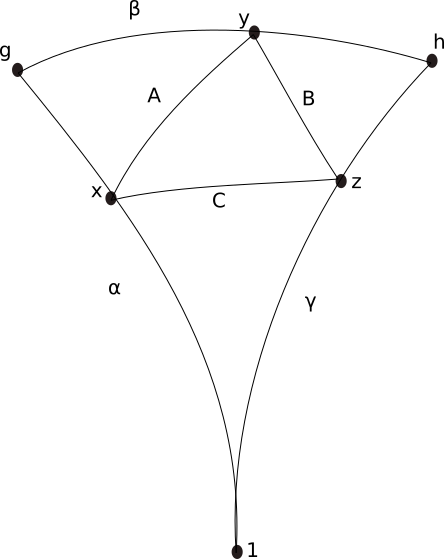
\includegraphics[scale=0.5]{treewidth.png}
	\caption*{}
\end{figure}



Ahora estamos listos para ver que $d(g,h) \le 3k$. Usamos la desigualdad triangular tres veces,
\begin{align*}
	d(g,h) & \le d(g,x) + d(x,z) + d(h,z) \\
	& \le d(x,y) + d(x,z) + d(y,z) \le 3k
\end{align*}
tal como queríamos ver.
\end{proof}

\begin{ej}
	Ejemplo de $PSL(2,\ZZ)$ o de algún otro grupo que sea un producto libre de grupos finitos.
\end{ej}


\section{Cuasisometrías.}


\begin{deff}
	Sean $(X,d_X),(Y,d_Y)$ espacios métricos. 
	Una \blue{cuasisometría} es una función $f:X \to Y$ tal que:
	\begin{itemize}
	\item[\textbf{Q1.}] Existe constante $A > 0$ tal que para todo par de puntos $x_1,x_2 \in X$ hace valer la siguientes desigualdades
	\[
	\frac{1}{A} d_X(x_1,x_2) - A \le d_Y(f(x_1),f(x_2)) \le A d_X(x_1,x_2) + A
	\]
	\item[\textbf{Q2.}] Existe una constante $C \ge 0$ tal que para todo punto $y \in Y$ debe existir $x \in X$ de manera que 
	\[
	d(y,f(x)) \le C
	\]
	\end{itemize}
 	Dos espacios métricos que se dicen \emph{cuasisométricos} si existe una cuasisometría entre ellos.
\end{deff}

\begin{obs}
	Si nos restringimos a que los espacios métricos sean grafos podemos redefinir una cuasisometría para que sea una función de los vértices de un grafo a los del otro.
	Esto es si tenemos dos grafos $\Gamma_1$ y $\Gamma_2$ entonces son cuasisométricos como espacios métricos si y solo si existe $f:V(\Gamma_1) \to V(\Gamma_2)$ tal que 
	\begin{itemize}
		\item Para todo $v,w \in V(\Gamma_1)$ existe constante $A > 0$ tal que 
		\[
		\frac{1}{A} d_X(v,w) - A \le d_Y(f(v),f(w)) \le A d_X(v,w) + A
		\]
		\item Existe una constante real $C \ge 0$ tal que para todo vértice $y \in V(\Gamma_2)$ existe $v \in V(\Gamma_1)$ tal que 
		\[
		d(y,f(v)) \le C
		\]
	\end{itemize}
	
	Para esto si tenemos una cuasisometría $g$ como espacios métrices definamos una sobre los vértices $f$ de la siguiente manera.
	Por cada vértice $v \in V(\Gamma_1)$ consideremos $g(v) \in \Gamma_2$. 
	Si $g(v) \in V(\Gamma_2)$ tomamos $f(v)=g(v)$.
	El otro caso es que $g(v)$ cae en el medio de alguna arista $xy \in E(\Gamma_2)$. 
	Supongamos que $d(g(v),x) \le \frac{1}{2}$ porque la distancia máxima con alguno de los vértices debe ser no más de $\frac{1}{2}$ porque justamente las aristas son isométricas con el intervalo $[0,1]$. 
	En este caso definamos $f(v) = x$.
	Notemos ahora que la distancia entre dos vértices por medio de $f$ a lo sumo aumenta. 
	Tenemos que 
	\[
		d(f(v),f(w) \le d (g(v),g(w)) + 1
	\]
	 para $v,w \in V(\Gamma_1)$ porque a lo sumo las imágenes por $g$ están a distancia $\frac{1}{2}$ de alguno de los vértices.
	De esta manera notemos que si tomamos la constante $C+1$ nos sirve.
	Para ver que la imagen es cuasidensa idénticamente tomando $C+1$ nos sirve.
	En definitiva $f$ definida de esta manera es una cuasisometría con constante $C+1$.	
\end{obs}

\begin{prop}
	Si existe $f:X \to Y$ cuasisometría entonces también debe haber $g:Y \to X$ cuasisometría.
\end{prop}
\begin{proof}
	Resultado estándar. Ver \cite{bridson2013metric}.
\end{proof}

Todo espacio métrico es cuasisométrico consigo mismo por medio de la identidad.
La composición de cuasisometrías también sigue siendo una cuasisometría.
Con esta proposición vemos que ser cuasisométricos es una relación de equivalencia entre los espacios métricos. 


Intuitivamente una cuasisometría entre espacios métricos nos dice que estos resultan ser bastante similares al menos desde cierta distancia. 
\medskip

\begin{ej}
Ejemplo de $\ZZ \times \ZZ$ para ver que no es cuasisométrico con un árbol o bien podría rehacer el ejemplo de la parte anterior.
\end{ej}

Todo grafo de Cayley lo podemos pensar como un espacio métrico tal como lo definimos en la sección \ref{seccion_treewidth}.  
Veamos que esto no depende de los generadores que hayamos elegido.

\begin{prop}
	Sea $G$ grupo \fg por $\Sigma$ y $\Delta$ conjuntos finitos entonces $\text{Cay}(G,\Sigma)$ y $\text{Cay}(G, \Delta)$ son cuasisométricos entre sí.
\end{prop}

\begin{proof}
	Resultado estándar. Ver \cite{bridson2013metric}.
\end{proof}



Así otra manera de pensar que un grafo de un grupo virtualmente libre es casi un árbol es pedirle que sea cuasisométrico con un árbol. 
Veamos que estas categorización es equivalente a pedirle que el treewidth sea finito que era la otra caracterización que habíamos obtenido anteriormente.

\begin{prop} \label{treewidth-inv}
	El treewidth finito es un invariante por cuasisometría para grafos con grado acotado uniformemente.
\end{prop}
%\begin{proof}[Intento de demo distinta. No salió]
%Si tenemos una cuasisometría $f:\Gamma_1 \to \Gamma_2$ tal que $\Gamma_1$ tiene treewidth finito $k \in \NN$, nos gustaría ver que $\Gamma_2$ también tiene treewidth finito.
%Dada la cuasisometría $f$ consideremos $C \ge A + B$.
%
%Partamos de una descomposición en un árbol $T$ para $\Gamma_1$.
%La idea es usar la cuasisometría para empujar esta descomposición a una (con bolsones posiblemente más grandes) en $\Gamma_2$.
%Por cada bolsón $X_t \subset V(\Gamma_1)$ vamos a considerar un bolsón en el otro grafo,
%\[
%Y_t = B(f(X_t),Ck) \cap V(\Gamma_2).
%\] 
%Esto es todos los vértices de $\Gamma_2$ que estén a distancia igual o menor que $Ck$ de la imagen del bolsón $X_t$ por medio de $f$. 
%Donde $k$ es la constante del treewidth del grafo $\Gamma_1$ y $C$ la constante de la cuasisometría anteriormente definida.
%
%Como ya sabemos que $T$ el grafo subyacente de la descomposición es un árbol basta ver que cumple las tres propiedades que debe cumplir toda descomposición \ref{desc-arbol}.
%
%\begin{enumerate}
%	\item Queremos ver que dado $v \in V(\Gamma_2)$ existe $t \in V(T)$ tal que $v \in Y_t$.
%	Por ser un embedding cuasisométrico debe existir $y \in \Gamma_1$ (no necesariamente algún vértice) tal que $d(f(y),v) \le C$. 
%	Tomemos $x \in V(\Gamma_1)$ de manera que $d(x,y) < 1$. 
%	Usando desigualdad triangular notemos que 
%	\[
%	d(f(x),v) \le d(f(x),f(y)) + d(v,f(y)) \le 2C
%	\]
%	donde $d(f(x),f(y)) \le C$ porque $f$ es una cuasisometría.
%	Mientras que la otra cota vale porque justamente así tomamos a $f(y)$. 
%	Como $k \le 2$ tenemos que $2C \le Ck$ y así vemos que $v \in Y_t$ tal como queríamos ver.
%	\item Dado una arista $vw \in E(\Gamma_2)$ veamos que $v, w \in Y_t$ para algún mismo bolsón $Y_t$.
%	Por la cuenta anterior sabemos que todo $v \in V(\Gamma_2)$ es tal que existe algún $x \in V(\Gamma_1)$ de manera que $d(f(x),v) \le C + 1$.
%	Si tomamos este mismo $x$ notemos que como $d(v,w) = 1$ entonces $d(w,x) \le C+2$. 
%	Esto nos dice que $v,w \in Y_t$ donde $Y_t$ es la bolsa correspondiente a $f(x)$. 
%	\item Sea $v \in Y_t \cap Y_s$ queremos ver que $v \in Y_r$ para todo $r$ en la geodésica que une $t$ con $s$ en el árbol $T$.
%	Alcanza con tomarnos $Y_t$ tal que exista $x \in V(\Gamma_1)$ con $x \in X_t$ de manera que $d(f(x),v) \le 2C$.	
%	Esto lo podemos hacer porque $f$ es una cuasisometría. 
%	Fijemos uno de los bolsones y veamos que para toda geodésicas que parten del vértice del árbol $t$ y terminan en $s$ son tales que todos los vértices $r \in V(T)$ que aparecen cumplen que $v \in Y_r$. 
%	Si no pudiéramos hacer esto tendríamos que nuestro grafo $T$ tiene un ciclo pero esto es absurdo puesto que es un árbol.
%	Supongamos que $sr$ es una arista de $T$ y $rt$ es otra arista.
%%	Los casos de una geodésica en general se reducen a este usando inducción en la longitud del camino.
%%	Sabemos que existe $z \in X_r \cap X_t$ por la proposición \ref{}. 
%%	De esta manera como $|X_t| \le k$ tenemos que $d(x,z) \le k$. 
%%	Usando que $f$ es una cuasisometría tenemos que $d(f(x),f(z) \le Ck$.
%%	
%%	Entonces veamos de acotar $d(f(z),v)$ y así concluir que $x \in Y_r$ tal como queríamos ver.
%%	Usando la desigualdad triangular,
%%	\[
%%	d(f(z),v) \le d(f(z),f()) + d(v,f(x)) \le Ck + C + 2
%%	\]
%%	y esto termina la demostración porque inductivamente lo podemos ver para cualquier $r$ en la geodésica.
%
%\red{Ahora creo que esto no es cierto. La tercera condición se rompa incluso en un ejemplo finito.}
%\end{enumerate}
%
%\end{proof}

\begin{proof}
	Si tenemos una cuasisometría $f:\Gamma_1 \to \Gamma_2$ tal que $\Gamma_2$ tiene treewidth finito $k \in \NN$, nos gustaría ver que $\Gamma_1$ también tiene esta propiedad.
	Consideremos $l$ tal que $d(f(v),f(w)) \le l$ para vértices $v,w \in V(\Gamma_1)$ que estén conectados por una arista.
	Esto lo podemos tomar porque al ser una cuasisometría 
	\[
	d(f(v),f(w)) \le C d(v,w) + C  \le 2C
	\]
	entonces basta con tomar $l \ge C+1$.
	
	Veamos de armarnos la descomposición en un árbol $T$ para $\Gamma_1$.	
	Tomaremos como árbol para descomposición al mismo $T$ que usamos para $\Gamma_2$.
	Sean $X_t$ los bolsones de esta descomposición. 
	Recordemos que por \ref{prop-vecinos-desc} si tomamos $N^l(X_t)$ los vecinos del bolsón $X_t$ que están a distancia no mayor a $l$ seguimos teniendo una descomposición.  
	Consideraremos los bolsones $Y_t = f^{-1}(N^l(X_t))$ de vértices en $\Gamma_1$. 
	
	Debemos ver que cumplen las tres propiedades.
	
	\begin{enumerate}
		\item[\textbf{T1.}] La primera se cumple puesto que los bolsones $X_t$ cubren $V(\Gamma_2)$. 
		De esta manera $\cup_{t \in T} N^l(X_t) = V(\Gamma_2)$ y por lo tanto tomando preimagen tenemos que
		\[
		\bigcup_{t \in V(T)} f^{-1} (N^l (X_t)) = \bigcup_{t \in V(T)} Y_t = f^{-1} (V(\Gamma_2)) = V(\Gamma_1)
		\] 
		donde usamos que la preimagen de la unión es la unión de las preimágenes.
		\item[\textbf{T2.}] La segunda condición usamos que si hay una arista $xy \in E(\Gamma_2)$ luego debe ser que $d(f(x),f(y)) \le l$ por como tomamos a $l$.
		De esta manera como $f(x) \in X_t$ para algún $t \in V(T)$, notemos que $f(y) \in N^l(X_t)$ también. 
		Tomando preimagen tenemos que $x,y \in f^{-1}(N^l(X_t))$ y esto es que justamente $x,y \in Y_t$ para un mismo $t \in V(T)$ tal como queríamos ver.		
		\item[\textbf{T3.}] Para la tercera condición si $x \in Y_t \cap Y_s$ queremos ver que $x \in Y_r$ para todo $r \in V(T)$ que aparezca en la geodésica de $s$ a $t$.
		Como la preimagen de una intersección es lo mismo que la intersección de las preimágenes entonces 
		\[
		x \in f^{-1}(N^l(X_t)) \cap f^{-1}(N^l(X_s)) = f^{-1}(N^l(X_t) \cap N^l (X_s)
		\]
		de esta manera debe existir $v \in V(\Gamma_2)$ tal que $v \in N^l(X_s) \cap N^l(X_t)$.
		Ahora usamos que esta es una descomposición sobre $\Gamma_2$ para notar que $v \in N^l(X_r)$.
		Tomando preimagen tenemos que $x \in Y_r$ tal como queríamos ver.
	\end{enumerate}
	
	Finalmente debemos ver que el tamaño de los bolsones está acotado uniformemente.
	Esto es que exista $k \in \NN$ tal que $|Y_t| \le k$ para todo $t \in V(T)$.
	Como $\Gamma_2$ tiene treewidth finito tenemos que $|X_t| \le M$ uniformemente para todo $y \in V(T)$ para cierta $M$. 
	Como el grado de los grafos está acotado uniformemente por alguna constante $d$ tenemos que 
	\[
	|N^l(X_t)| \le d^l |X_t| \le d^l M.
	\]
	Finalmente notemos que al ser $f$ una cuasisometría tenemos que $|f^{-1}(v)| \le k$ para todo $v \in V(\Gamma_2)$.
	Esto lo podemos ver porque si $f(x) = v = f(y)$ entonces
	\[
	\frac{1}{C}d(x,y) - C \le d( f(x), f(y) ) = 0 \implies d(x,y) \le C^2 < \infty
	\]
	y esta cota es uniforme para todo $v \in \Gamma_2$. 
	Así vemos que,
	\[
	|Y_t| = |f^{-1}(N^l(X_t))| \le C^2 d^l M < \infty
	\]
	y tomamos $k$ suficientemente grande para que haga valer esto.
	Concluímos así que la descomposición que nos armamos para $\Gamma_1$ tiene treewidth finito.
\end{proof}

A partir de este resultado podemos ver que la otra manera que teníamos de pensar a los grafos que se parecen a árboles resulta ser más débil. 
El siguiente resultado lo demostramos en el caso general de un grafo tal que los grados de sus vértices están acotados uniformemente. 
Como caso particular tenemos los grafos de Cayley de grupos finitamente generados.


\begin{prop} 
	Un grafo $X$ de grado acotado uniformemente cuasisométrico con un árbol tiene treewidth finito.
\end{prop}
\begin{proof}	
%Para la ida veamos de armarnos la cuasisometría a partir de la descomposición en árbol del grafo $X$. 
%Definamos entonces la cuasisometría $q: T \to X$ a partir de mandar $t \to x_t$ donde $x_t \in X_t$ es algún elemento del bolsón correspondiente a $t \in V(T)$ que sabemos que no es vacío. 
%Esta función es una cuasisometría con constante $C=1$ y $A = bs(T) + 1$.
%
%Hay que ver la distancia dentro de un bolsón esté controlada.
%Si los bolsones los tomamos conexos \ref{} entonces notemos que la mayor distancia posible es...
Dado que el grafo $X$ es cuasisométrico a un árbol $T$, por la observación \ref{desc-arbol-arbol} este tiene treewidth exactamente 1.
Por la proposición anterior \ref{treewidth-inv} como es un invariante por cuasisometría vemos que $X$ debe tener treewidth finito tal como queríamos ver.
\end{proof}

\begin{coro}
	Todo grupo independiente de contexto es tal que su grafo de Cayley es cuasisométrico a un árbol.
\end{coro}
\begin{proof}
	Por \ref{teo_schupp_muller_ic_desc} todo grupo independiente de contexto tiene treewidth finito y usando la proposición recién demostrada concluímos que su grafo de Cayley es cuasisométrico a un árbol.
\end{proof}


\begin{prop}\label{cuasisometria-subgrupo-ind-finito}
	Sea $G$ grupo \fg entonces si $H$ es un subgrupo de índice finito resulta que son cuasisométricos.
\end{prop}
\begin{proof}
	Resultado estándar pero no tan elemental de demostrar. 
	Es un corolario de Milnor Schwarz.
	Ver \cite{loh2017geometric}.
\end{proof}

Esto nos dice que todo grupo es cuasisométrico con los subgrupos de índice finito. 
De esta manera obtenemos el siguiente resultado,

\begin{prop}
	Todo grafo de Cayley de un grupo virtualmente libre es cuasisométrico a un árbol.
\end{prop}

\begin{proof}
	Si $G$ es virtualmente libre entonces existe $F \le G$ grupo libre de índice finito.
	Por la prop anterior \ref{cuasisometria-subgrupo-ind-finito} tenemos que el grafo de Cayley de $G$ es cuasisométrico con el de $H$.
	Por el resultado \ref{} sabemos que los grafos de grupos libres son árboles y así queda demostrada la proposición.
\end{proof}



\end{document}